\section{Semantics}
\label{sec:conanal}
This section will define the scope and type rules of WAR.
	\subsection{Scope rules}
		A scope is a block of code, in WAR one is able to denote a new scope by using $\{$ to start the scope and $\}$.
		A scope placed inside another scope is called a {\it nested scope}. A {\it scope level} denotes how nested a given scope is,
		e.g. identifiers at scope level 0 is outside any scope, identifiers at scope level 1 is inside one scope etc.
		\begin{lstlisting}
		Scope
		{
			//Scope level 1
			identifier = 2
			Scope
			{
				//Scope level 2
				identifier = 2
			}
		}
		\end{lstlisting}
		
		Scope rules dictate the accessibility of identifiers from one scope to another\cite{SPOBOG}.
	
	%These are the rules that defines how the identifiers must be read, and where to declare them - also known as identification.
	The WAR language has a nested block-structure which means we may have constants or variables can be defined in multiple scope levels. 
	Scope rules may be defined in levels, such that a declaration in the outermost block is at scope level 1, however, since the language has no declaration of variables, only constants, it works the same way. If you declare the $Size$ of a regiment at scope level 1, you can use $Size$ in all the higher scope levels. Declarations inside a block are referred to as being local in that block.

	The use of a nested block structure we follow some basic scope rules:
	\begin{wrapfigure}{r}{0.5\textwidth}
		\begin{center}
			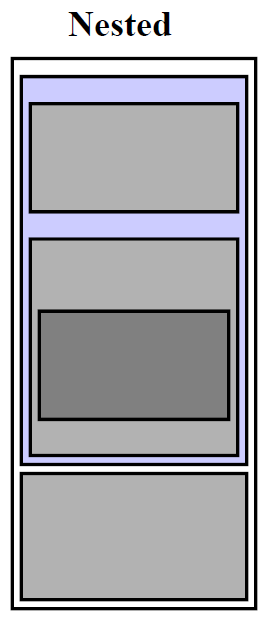
\includegraphics[scale=0.5]{rapport/5/figures/nested_block_structure}
		\end{center}	
		\caption{Illustration of the nested block structure}
		\label{nested_block_structure}
	\end{wrapfigure}


	%INCLUDE BIBLIOGRAPHY!!!	
	\begin{itemize}
	\item No identifier may be declared more than once within the same block (at the same level) %SPO
	\item For any applied occurrence there must be a corresponding occurrence, either within the same block or block which is higher up in the nesting. %SPO
	%INCLUDE BIBL...
	\end{itemize}
	
	
	Referring to figure \ref{nested_block_structure} which demonstrates the functioning of a nested block structure visually. Initially we consider how the nested block structure works in general and later an example of how the nested block structure works in the WAR programming language.
	
	One can have as many and as few blocks as needed, and every sub-block of an existing block, can use all the variables that have been declared in blocks over itself. 
	
	
	%Her kommer noget kode af vores egen for at beskrive hvordan nested block structure virker hos os.
		
\newpage
	
	
%Page 142 i Brown!! :D